\begin{frame}
	\frametitle{Parameter selection}
	
	\begin{itemize}
		\item many EvoSuite parameter
		\item nearly infinite possible combinations
		\item small-scale experiments
		\item using small sample $S_3$
	\end{itemize}
	
\end{frame}

\begin{frame}
	\frametitle{Influence on runtime}
	\begin{figure}
		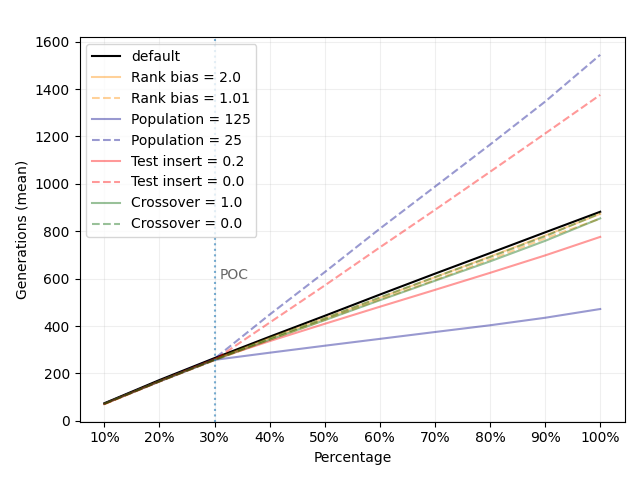
\includegraphics[height=0.9\textheight]{figures/generations_parameter}
	\end{figure}	
\end{frame}

\begin{frame}
	\frametitle{Event probability}
	
	\begin{columns}[c]
		
		\column{.35\textwidth}
		
		\begin{itemize}
			\item runtime in relation to event probability
			\begin{itemize}
				\item insert
				\item mutate
				\item crossover
			\end{itemize}
			\item trade-off
			\begin{itemize}
				\item fitness evaluation
				\item event occurrence
			\end{itemize}
		\end{itemize}
		
		\column{.60\textwidth}
		\begin{equation}
			P_{adj}(e) = \frac{n_1 P_1(e) + n_2 P_2(e)}{n_1 + n_2}
		\end{equation}
		
		\begin{equation}
			\hat{P}(e) = \sum_{i=k}^n \frac{n!}{i!(n-i)!} P_{adj}(e)^i (1-P_{adj}(e))^{n-i}
		\end{equation}
		
	\end{columns}
	
\end{frame}

\begin{frame}
	\frametitle{Component selection}
	
	\begin{table}
		\centering
		\resizebox{\textwidth}{!}{\begin{tabular}{lll|lll|lll|ll}
\hline
                           &              &            & \multicolumn{3}{l|}{$P_{adj}$}                & \multicolumn{3}{l|}{$\hat{P}$ for $k = 5$}                 &            &            \\
configuration              & gen.         & n          & mut.          & cross.        & ins.          & mut.          & cross.          & ins.                     & $n\_+$       & $n\_-$       \\ \hline
default                    & 853          & 9          & 0.95          & 0.68          & 0.05          & 1.0           & 0.87            & 0.0                      &          &          \\
p = 25                     & 1,263        & 13         & 0.96          & 0.69          & 0.04          & 1.0           & 1.0 $\nearrow$  & 0.0                      & 0          & 0          \\
p = 125                    & 572          & 6          & 0.95          & 0.68          & 0.04          & 0.77          & 0.15            & 0.0                      & 3          & 0          \\
cr = 0.0                   & 841          & 8          & 0.95          & 0.0           & 0.05          & 1.0           & 0.0             & 0.0                      & 1          & 0          \\
cr = 1.0                   & 849          & 8          & 0.95          & 0.95          & 0.05          & 1.0           & 1.0 $\nearrow$  & 0.0                      & 0          & 0          \\
bias = 2.0                 & 912          & 9          & 0.95          & 0.68          & 0.05          & 1.0           & 0.88 $\nearrow$ & 0.0                      & 1          & 0          \\
bias = 1.01                & 824          & 8          & 0.95          & 0.68          & 0.05          & 1.0           & 0.77            & 0.0                      & 0          & 0          \\
pti = 0.0                  & 1,154        & 12         & 1.0           & 0.75          & 0.0           & 1.0           & 1.0 $\nearrow$  & 0.0                      & 0          & 4          \\
pti = 0.2                  & 770          & 8          & 0.92          & 0.63          & 0.08          & 1.0           & 0.66            & 0.0                      & 0          & 0          \\
p = 10, pti = 5.0          & 912          & 9          & 0.58          & 0.13          & 0.42          & 0.69          & 0.0             & 0.31 $\nearrow$          & 3          & 0          \\
\textbf{p = 25, pti = 1.0} & \textbf{777} & \textbf{8} & \textbf{0.75} & \textbf{0.38} & \textbf{0.25} & \textbf{0.89} & \textbf{0.14}   & \textbf{0.03 $\nearrow$} & \textbf{4} & \textbf{0} \\ \hline
\end{tabular}}
	\end{table}
	
\end{frame}